\section{ATAN Inverse Trigonometric Arctangent Function}

\subsection{Usage}

Computes the \verb|atan| function for its argument.  The general
syntax for its use is
\begin{verbatim}
  y = atan(x)
\end{verbatim}
where \verb|x| is an \verb|n|-dimensional array of numerical type.
Integer types are promoted to the \verb|double| type prior to
calculation of the \verb|atan| function.  Output \verb|y| is of the
same size and type as the input \verb|x|, (unless \verb|x| is an
integer, in which case \verb|y| is a \verb|double| type).  
\subsection{Function Internals}

Mathematically, the \verb|atan| function is defined for all 
arguments \verb|x| as
\[
   \mathrm{atan} x \equiv \frac{i}{2}\left(\log(1-i x) - \log(i x + 1)\right).
\]
For real valued variables \verb|x|, the function is computed directly using 
the standard C library's numerical \verb|atan| function. For both 
real and complex arguments \verb|x|, note that generally

\[
    \mathrm{atan}(\tan(x)) \neq x,
\]
 due to the periodicity of \verb|tan(x)|.
\subsection{Example}

The following code demonstates the \verb|atan| function over the range 
\verb|[-1,1]|.
\begin{verbatim}
--> t = linspace(-1,1);
--> plot(t,atan(t))
\end{verbatim}


\centerline{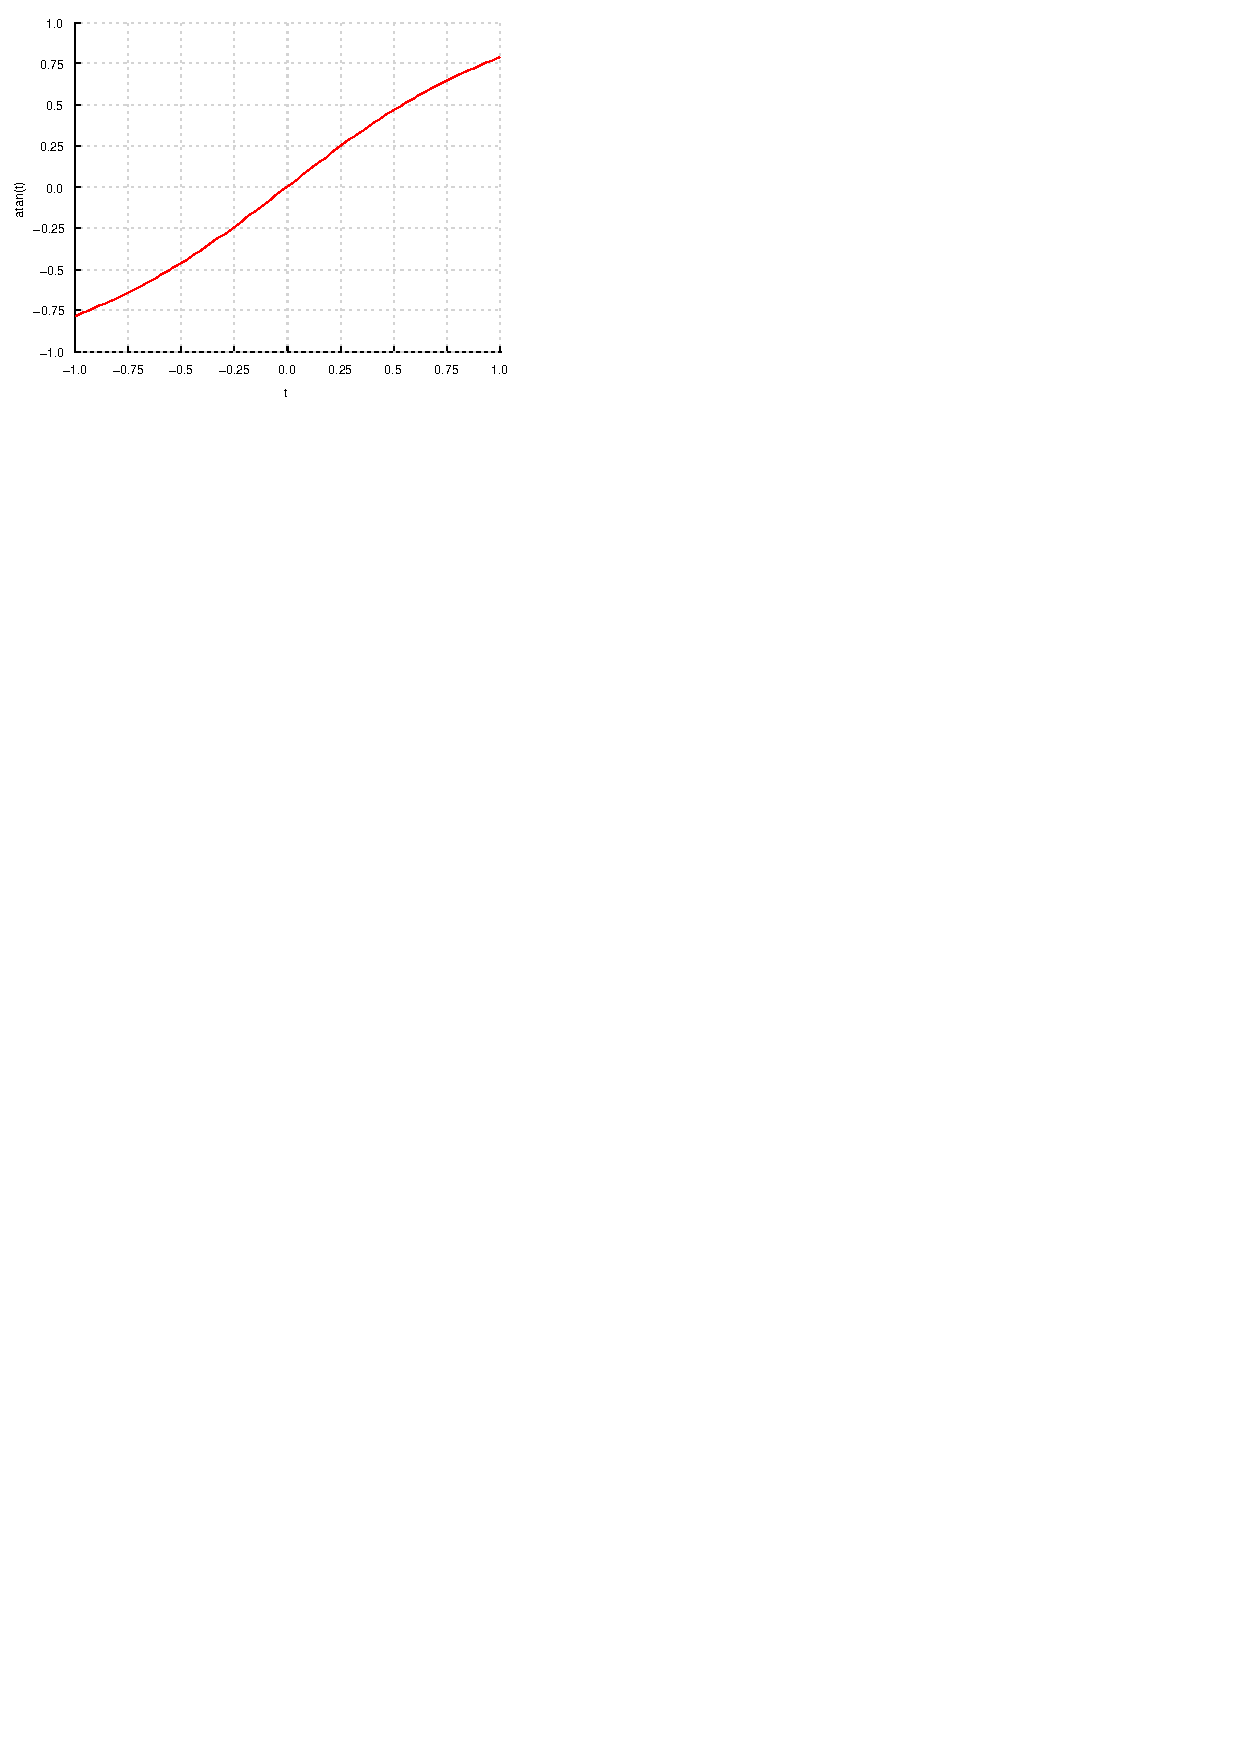
\includegraphics[width=8cm]{atanplot}}

